% ****************************************************************************************
% *********************        SISTEMAS OPERATIVOS            ****************************
% ****************************************************************************************


% =======================================================
% =======         HEADER FOR DOCUMENT        ============
% =======================================================
    % *********   DOCUMENT ITSELF   **************
    \documentclass[12pt, fleqn]{report}                             %Type of docuemtn and size of font and left eq
    \usepackage[margin=1.2in]{geometry}                             %Margins and Geometry pacakge
    \usepackage{ifthen}                                             %Allow simple programming
    \usepackage{hyperref}                                           %Create MetaData for a PDF and LINKS!
    \hypersetup{pageanchor=false}                                   %Solve 'double page 1' warnings in build
    \setlength{\parindent}{0pt}                                     %Eliminate ugly indentation
    \author{Oscar Andrés Rosas}                                     %Who I am

    % *********   LANGUAJE AND UFT-8   *********
    \usepackage[spanish]{babel}                                     %Please use spanish
    \usepackage[utf8]{inputenc}                                     %Please use spanish - UFT
    \usepackage[T1]{fontenc}                                        %Please use spanish
    \usepackage{textcmds}                                           %Allow us to use quoutes
    \usepackage{changepage}                                         %Allow us to use identate paragraphs

    % *********   MATH AND HIS STYLE  *********
    \usepackage{ntheorem, amsmath, amssymb, amsfonts}               %All fucking math, I want all!
    \usepackage{mathrsfs, mathtools, empheq}                        %All fucking math, I want all!
    \usepackage{centernot}                                          %Allow me to negate a symbol
    \decimalpoint                                                   %Use decimal point

    % *********   GRAPHICS AND IMAGES *********
    \usepackage{graphicx}                                           %Allow to create graphics
    \usepackage{wrapfig}                                            %Allow to create images
    \graphicspath{ {Graphics/} }                                    %Where are the images :D

    % *********   LISTS AND TABLES ***********
    \usepackage{listings}                                           %We will be using code here
    \usepackage[inline]{enumitem}                                   %We will need to enumarate
    \usepackage{tasks}                                              %Horizontal lists
    \usepackage{longtable}                                          %Lets make tables awesome
    \usepackage{booktabs}                                           %Lets make tables awesome
    \usepackage{tabularx}                                           %Lets make tables awesome
    \usepackage{multirow}                                           %Lets make tables awesome
    \usepackage{multicol}                                           %Create multicolumns


    % *********   HEADERS AND FOOTERS ********
    \usepackage{fancyhdr}                                           %Lets make awesome headers/footers
    \pagestyle{fancy}                                               %Lets make awesome headers/footers
    \setlength{\headheight}{16pt}                                   %Top line
    \setlength{\parskip}{0.5em}                                     %Top line
    \renewcommand{\footrulewidth}{0.5pt}                            %Bottom line

    \lhead{                                                         %Left Header
        \hyperlink{chapter.\arabic{chapter}}                        %Make a link to the current chapter
        {\normalsize{\textsc{\nouppercase{\leftmark}}}}             %And fot it put the name
    }

    \rhead{                                                         %Right Header
        \hyperlink{section.\arabic{chapter}.\arabic{section}}       %Make a link to the current chapter
            {\footnotesize{\textsc{\nouppercase{\rightmark}}}}      %And fot it put the name
    }

    \rfoot{\textsc{\small{\hyperref[sec:Index]{Ve al Índice}}}}     %This will always be a footer  

    \fancyfoot[L]{                                                  %Algoritm for a changing footer
        \ifthenelse{\isodd{\value{page}}}                           %IF ODD PAGE:
            {\href{https://compilandoconocimiento.com/yo/}          %DO THIS:
                {\footnotesize                                      %Send the page
                    {\textsc{Oscar Andrés Rosas}}}}                 %Send the page
            {\href{https://compilandoconocimiento.com}              %ELSE DO THIS: 
                {\footnotesize                                      %Send the author
                    {\textsc{Compilando Conocimiento}}}}            %Send the author
    }
    
    
    
% ========================================
% ===========   COMMANDS    ==============
% ========================================

    % =====  GENERAL TEXT  ==========
    \newcommand \Quote {\qq}                                        %Use: \Quote to use quotes
    \newcommand \Over {\overline}                                   %Use: \Bar to use just for short
    \newcommand \ForceNewLine {$\Space$\\}                          %Use it in theorems for example
    
    \newenvironment{Indentation}[1][0.75em]                         %Use: \begin{Inde...}[Num]...\end{Inde...}
    {\begin{adjustwidth}{#1}{}}                                     %If you dont put nothing i will use 0.75 em
    {\end{adjustwidth}}                                             %This indentate a paragraph
    \newenvironment{SmallIndentation}[1][0.75em]                    %Use: The same that we upper one, just 
    {\begin{adjustwidth}{#1}{}\begin{footnotesize}}                 %footnotesize size of letter by default
    {\end{footnotesize}\end{adjustwidth}}                           %that's it


    % =====  GENERAL MATH  ==========
    \DeclareMathOperator \Space {\quad}                             %Use: \Space for a cool mega space
    \DeclareMathOperator \MiniSpace {\;}                            %Use: \Space for a cool mini space
    \newcommand \Such {\MiniSpace|\MiniSpace}                       %Use: \Such like in sets
    \newcommand \Also {\MiniSpace \text{y} \MiniSpace}              %Use: \Also so it's look cool
    \newcommand \Remember[1]{\Space\text{\scriptsize{#1}}}          %Use: \Remember so it's look cool

    \newtheorem{Theorem}{Teorema}[section]                          %Use: \begin{Theorem}[Name]\label{Nombre}...
    \newtheorem{Corollary}{Colorario}[Theorem]                      %Use: \begin{Corollary}[Name]\label{Nombre}...
    \newtheorem{Lemma}[Theorem]{Lemma}                              %Use: \begin{Lemma}[Name]\label{Nombre}...
    \newtheorem{Definition}{Definición}[section]                    %Use: \begin{Definition}[Name]\label{Nombre}...

    \newcommand{\Set}[1]{\left\{ \MiniSpace #1 \MiniSpace \right\}} %Use: \Set {Info}
    \newcommand{\Brackets}[1]{\left[ #1 \right]}                    %Use: \Brackets {Info} 
    \newcommand{\Wrap}[1]{\left( #1 \right)}                        %Use: \Wrap {Info} 
    \newcommand{\pfrac}[2]{\Wrap{\dfrac{#1}{#2}}}                   %Use: Put fractions in parentesis

    \newenvironment{MultiLineEquation}[1]                           %Use: To create MultiLine equations
        {\begin{equation}\begin{alignedat}{#1}}                     %Use: \begin{Multi..}{Num. de Columnas}
        {\end{alignedat}\end{equation}}                             %And.. that's it!
    \newenvironment{MultiLineEquation*}[1]                          %Use: To create MultiLine equations
        {\begin{equation*}\begin{alignedat}{#1}}                    %Use: \begin{Multi..}{Num. de Columnas}
        {\end{alignedat}\end{equation*}}                            %And.. that's it!


    % =====  LOGIC  ==================
    \DeclareMathOperator \doublearrow {\leftrightarrow}             %Use: \doublearrow for a double arrow
    \newcommand \lequal {\MiniSpace \Leftrightarrow \MiniSpace}     %Use: \lequal for a double arrow
    \newcommand \linfire {\MiniSpace \Rightarrow \MiniSpace}        %Use: \lequal for a double arrow
    \newcommand \longto {\longrightarrow}                           %Use: \longto for a long arrow

    % =====  NUMBER THEORY  ==========
    \DeclareMathOperator \Naturals  {\mathbb{N}}                     %Use: \Naturals por Notation
    \DeclareMathOperator \Primes    {\mathbb{P}}                     %Use: \Naturals por Notation
    \DeclareMathOperator \Integers  {\mathbb{Z}}                     %Use: \Integers por Notation
    \DeclareMathOperator \Racionals {\mathbb{Q}}                     %Use: \Racionals por Notation
    \DeclareMathOperator \Reals     {\mathbb{R}}                     %Use: \Reals por Notation
    \DeclareMathOperator \Complexs  {\mathbb{C}}                     %Use: \Complex por Notation

    % === LINEAL ALGEBRA & VECTORS ===
    \DeclareMathOperator \LinealTransformation {\mathcal{T}}        %Use: \LinealTransformation for a cool T
    \newcommand{\Mag}[1]{\left| #1 \right|}                         %Use: \Mag {Info} 

    \newcommand{\pVector}[1]{                                       %Use: \pVector {Matrix Notation} use parentesis
        \ensuremath{\begin{pmatrix}#1\end{pmatrix}}                 %Example: \pVector{a\\b\\c} or \pVector{a&b&c} 
    }
    \newcommand{\lVector}[1]{                                       %Use: \lVector {Matrix Notation} use a abs 
        \ensuremath{\begin{vmatrix}#1\end{vmatrix}}                 %Example: \lVector{a\\b\\c} or \lVector{a&b&c} 
    }
    \newcommand{\bVector}[1]{                                       %Use: \bVector {Matrix Notation} use a brackets 
        \ensuremath{\begin{bmatrix}#1\end{bmatrix}}                 %Example: \bVector{a\\b\\c} or \bVector{a&b&c} 
    }
    \newcommand{\Vector}[1]{                                        %Use: \Vector {Matrix Notation} no parentesis
        \ensuremath{\begin{matrix}#1\end{matrix}}                   %Example: \Vector{a\\b\\c} or \Vector{a&b&c}
    }

    % MATRIX
    \makeatletter                                                   %Example: \begin{matrix}[cc|c]
    \renewcommand*\env@matrix[1][*\c@MaxMatrixCols c] {             %WTF! IS THIS
        \hskip -\arraycolsep                                        %WTF! IS THIS
        \let\@ifnextchar\new@ifnextchar                             %WTF! IS THIS
        \array{#1}                                                  %WTF! IS THIS
    }                                                               %WTF! IS THIS
    \makeatother                                                    %WTF! IS THIS

    % TRIGONOMETRIC FUNCTIONS
    \newcommand{\Cos}[1]{\cos\Wrap{#1}}                             %Simple wrappers
    \newcommand{\Sin}[1]{\sin\Wrap{#1}}                             %Simple wrappers

    % === COMPLEX ANALYSIS ===
    \newcommand \Cis[1]  {\Cos{#1} + i \Sin{#1}}                    %Use: \Cis for cos(x) + i sin(x)
    \newcommand \pCis[1] {\Wrap{\Cis{#1}}}                          %Use: \pCis for the same ut parantesis
    \newcommand \bCis[1] {\Brackets{\Cis{#1}}}                      %Use: \bCis for the same to Brackets

    % === CALCULUS ===
    \newcommand \Partial[2] {\dfrac{\partial #1}{\partial #2}}      %Use: \Partial for simple use

    % =====  GENERAL COLOR  =========
    \definecolor{TealMD}{HTML}{009688}                              %Use: Color :D        
    \definecolor{IndigoMD}{HTML}{3F51B5}                            %Use: Color :D
    \definecolor{Green100MD}{HTML}{DCEDC8}                          %Use: Color :D
    \definecolor{Blue300MD}{HTML}{64B5F6}                           %Use: Color :D
    \definecolor{DeepPurpleMD}{HTML}{673AB7}                        %Use: Color :D
    \definecolor{BlueGrey100MD}{HTML}{CFD8DC}                       %Use: Color :D
    \definecolor{BlueGrey800MD}{HTML}{37474F}                       %Use: Color :D
    \definecolor{BlueGrey200MD}{HTML}{B0BEC5}                       %Use: Color :D
    \definecolor{Lime300MD}{HTML}{E6EE9C}                           %Use: Color :D

    \newenvironment{ColorText}[1]{                                  %Use: \begin{ColorText}
        \leavevmode\color{#1}\ignorespaces}                         %That's is!


    % =====  CODE EDITOR =========
    \lstdefinestyle{CompilandoStyle} {                              %This is Code Style
        backgroundcolor=\color{BlueGrey800MD},                      %Background Color  
        basicstyle=\tiny\color{white},                              %Font color
        commentstyle=\color{BlueGrey200MD},                         %Comment color
        stringstyle=\color{Lime300MD},                              %String color
        keywordstyle=\color{Blue300MD},                             %keywords color
        numberstyle=\tiny\color{TealMD},                            %Size of a number
        frame=shadowbox,                                            %Adds a frame around the code
        breakatwhitespace=true,                                     %Style   
        showstringspaces=false,                                     %Hate those spaces                  
        breaklines=true,                                            %Style                   
        keepspaces=true,                                            %Style                   
        numbers=left,                                               %Style                   
        numbersep=10pt,                                             %Style 
        xleftmargin=\parindent,                                     %Style 
        tabsize=4                                                   %Style 
    }
 
    \lstset{style=CompilandoStyle}                                  %Use this style





% =====================================================
% ============        COVER PAGE       ================
% =====================================================
\begin{document}
\begin{titlepage}

    \center
    % ============ UNIVERSITY NAME AND DATA =========
    \textbf{\textsc{\Large Proyecto Compilando Conocimiento}}\\[1.0cm] 
    \textsc{\Large Ciencias de la Computación}\\[1.0cm] 

    % ============ NAME OF THE DOCUMENT  ============
    \rule{\linewidth}{0.5mm} \\[1.0cm]
        { \huge \bfseries Sistemas Operativos}\\[1.0cm] 
    \rule{\linewidth}{0.5mm} \\[2.0cm]
    
    % ====== SEMI TITLE ==========
    {\LARGE Una Pequeña (Gran) Introducción}\\[7cm] 
    
    % ============  MY INFORMATION  =================
    \begin{center} \large
    \textbf{\textsc{Autores:}}\\
        Rosas Hernandez Oscar Andrés    \\
        Lopez Manriquez Angel           \\
        Gonzalez Nuñez Daniel Adrian
    \end{center}

    \vfill

\end{titlepage}

% =====================================================
% ========                INDICE              =========
% =====================================================
\tableofcontents{}
\label{sec:Index}

\clearpage




% //////////////////////////////////////////////////////////////////////////////////////////////////////////
% ///////////////////////////////////              INTRODUCCION            /////////////////////////////////
% //////////////////////////////////////////////////////////////////////////////////////////////////////////
\part{Una Introducción}
\clearpage


    % ===============================================================================
    % ===================           DEFINICIONES               ======================
    % ===============================================================================
    \chapter{Introducción}

        % ==============================================
        % ========    REPOSITORIO DE DATOS     =========
        % ==============================================
        \clearpage
        \section{¿Qué es un Sistema Operativo?}
            
            Los sistemas operativos surgen como una solución a la problematica de la 
            \textbf{ administración de un equipo de computo}, de forma tal que fuese más sencillo
            trabajar con el y aprovechar al máximo sus recursos.
    
            \Quote{Un sistema operativo es un programa encargado de controlar todos lor recursos de
            una computadora}

            \subsection{Definición Formal}

                \Quote{Un sistema operativo es un software de base compuesto por un conjunto
                de administradores encargados de la administración (valga la redundancia) de cada uno de
                los recursos de un equipo de coputo de forma rápida y eficiente.}


            \subsection{Características}

                \begin{itemize}
                    \item 
                        \textbf{Un sistema operativo es un software de base} debido a que es una plataforma que permite
                        la creación y ejecución de aplicaciones desarrolladas para el propio sistema.
                        Como software de base, el sistem operativo ofrece interfaces para la creación o ejecución
                        de las aplicaciones desarrolladas.

                        Incluso mucha gente ve al sistema operativo como una biblioteca estandar.

                    \item
                        Un sistema operativo esta compuesto de un conjunto de administradores, los cuales controlan
                        todos los recursos del equipo de computo, estos administradores son: 

                        \begin{itemize}
                            \item Administrador de Procesos
                            \item Admin. de Memoria 
                            \item Admin. de Entrada / Salida 
                            \item Admin. de Archivos 
                            \item Admin. de Red 
                        \end{itemize}

                    \item
                        Un sistema operativo debe ejecutarse lo más rapido posible, evitando quitarle tiempo de
                        procesamiento a las aplicaciones de los usuarios, por otro lado debe administrar cada uno
                        de los recursos del equipo de cómputo de forma eficiente, maximizando el uso de cada
                        recurso controlado. 
                        La rápidez y eficiencia es uno de los principales u objetivos que un Sistema Operativo debe
                        cumplir durante su ejecución.
            
                \end{itemize}
       

        % ==============================================
        % ========    TIPO DE SISTEMAS         =========
        % ==============================================
        \section{Tipo de Sistemas}

            \subsubsection{Sistemas Genéricos:}
            \begin{itemize}
                \item Por lotes sencillos
                \item Por lotes multiprogramados
                \item De tiempo compartido
            \end{itemize}

            \subsubsection{Sistemas Especializados:}
            \begin{itemize}
                \item Distribuidos: En estos los procesadores no comparten el mismo reloj ni memoria, son sistemas
                    debilmente acomplados
                \item Paralelos: Los procesadores comparten los recursos como la memoria, son sistemas fuertemente
                    acomplados
            \end{itemize}     

        % ==============================================
        % ========      TERMINOS COMUNES       =========
        % ==============================================
        \clearpage
        \section{Terminos Básicos}

            \begin{itemize}
                \item
                    \textbf{Spooling: }

                    Spool significa \Quote{Simultaneous Peripheral Operation On-Line}.

                    En realidad, lo que sucede aquí es que hay buffer para almacenar los datos,
                    por lo general el disco.

                    Los dispositivos de entrada / salida no pueden trabajar a la velocidad de una CPU.
                    Por lo tanto, la salida de la CPU se almacenará en este spool (buffer) y los
                    dispositivos de entrada / salida pueden tomar la salida de este buffer como y cuando
                    se requiera de acuerdo a su velocidad.

                    Por lo tanto, la CPU no está vinculada a este dispositivo de entrada / salida y
                    puede realizar otras operaciones.
                    Gracias al spooling podemos mantener la CPU y los dispositivos de entrada y salida
                    trabajando a altas velocidades sin esperar el uno al otro.

                \item
                    \textbf{Reserva de Trabajo: }

                    Conjunto de trabajos en el disco listos para ser ejecutados por la CPU

                \item
                    \textbf{Planificación de Trabajo: }

                    Es la técnica que se encarga de seleccionar cual será el siguiente trabajo
                    ejecutado en la CPU.

                \item
                    \textbf{Multiprogramación: }

                    Técnica utilizada para almacenar múltiples trabajos simultáneamente en la 
                    memoria física (RAM).

                \item
                    \textbf{Tiempo Compartido: }

                    Técnica utilizada para asignar un tiempo de ejecución a cada proceso
                    lo suficientemente corto para conmutar entre ellos.

                    El sistema de tiempo compartido es donde cada proceso se asigna un período de
                    tiempo determinado y el proceso tiene que terminar su finalización dentro de ese
                    lapso de tiempo.

                    Si no se logra completar su ejecución, entonces el control de CPU pasa al
                    próximo proceso.

                \item
                    \textbf{Concurrencia: }

                    Técnica utilizada ejecutar múltiples trabajos bajo la apariencia de
                    simultaneidad o paralelismo mediante una ejecución secuencial.

                \item
                    \textbf{Memoria Virtual: }

                    Técnica utilizada para aumentar o extender la memoria física (RAM) mediante
                    el uso de una pequeña región de disco.

                \item
                    \textbf{Sistema de Archivos: }

                    Estructura de almacenamiento de información mediante entes llamados
                    archivos y directorios.

                \item
                    \textbf{Sistemas Paralelos: }

                    Sistemas utilizados para el multiprocesamiento compuesto por un conjunto
                    de procesadores que comparten el reljo, memoria y buses del equipo, por lo
                    que se conocen como fuertemente acoplados.

                \item
                    \textbf{Sistemas Distribuidos: }

                    istemas utilizados para el multiprocesamiento compuesto por un conjunto
                    de sistemas de cómputo completo que manejan de forma independiente cosas
                    como el reloj, la memoria o los buses. Por esto se le conoce como debilmente
                    acoplados.

            \end{itemize}



        % ===============================================================================
        % ===========          PARTES DEL SISTEMA OPERATIVO           ===================
        % ===============================================================================
        \clearpage
        \section{Partes del Sistema Operativo}

            % ==============================================
            % =============    VISTA GENERAL    ============
            % ==============================================
            \subsection{Vista General}

                Un Sistema Operativo como cualquier otro software sigue un modelo de ingeniería de
                software para su diseño y construcción, en modelo que se usa es el denominado por capas,
                este modelo nos dice que cada capa se encarga de realizar una funcionalidad concreta
                dentro del sistema operativo.

                Un sistema operativo normalmente está integrado por las siguientes capas:
                \begin{itemize}
                    \item Hardware
                    \item Kernel
                    \item Servicios        
                    \item Aplicaciones
                \end{itemize}  

                Estas capas para llevar a cabo sus funciones requieren comunicarse con cada adyacentes,
                para lograr esta comunicación se usan las interfaces,
                estas son:
                \begin{itemize}
                    \item Interfaz de Comandos
                    \item Interfaz de Llamafas al Sistema
                    \item Interfaz de Interrupciones        
                \end{itemize}  


                Graficamente las podemos ver como:

                \begin{figure}[h!]
                    \centering
                    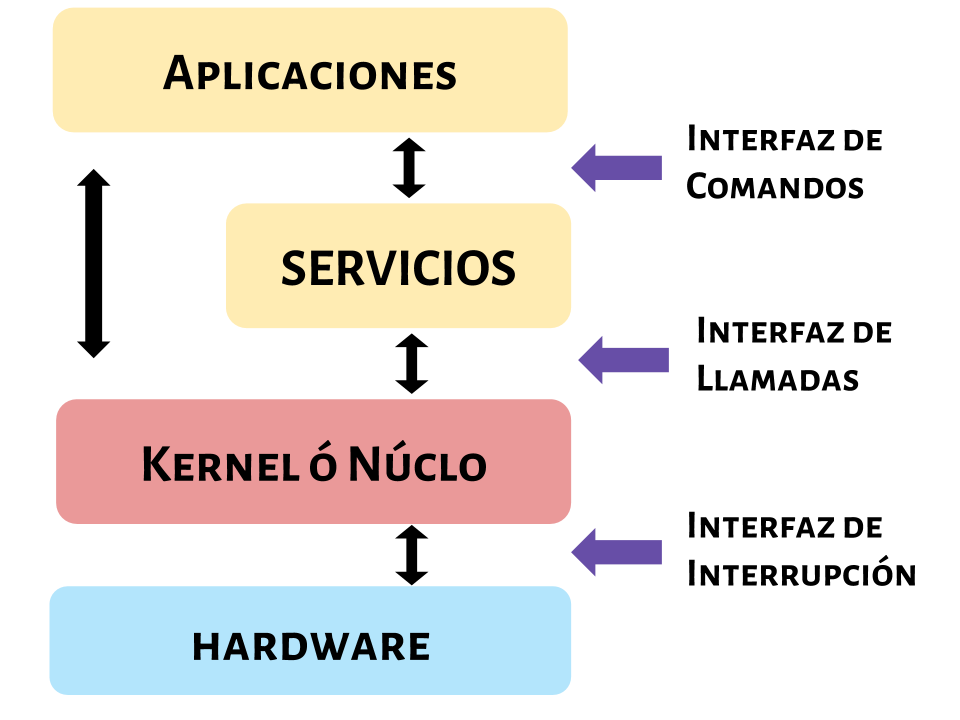
\includegraphics[width=0.55\textwidth]{Capas}
                \end{figure}

            % ==============================================
            % =============        CAPAS        ============
            % ==============================================
            \clearpage
            \subsection{Capas}    

                \begin{itemize}
                    \item
                        \textbf{Capa de Aplicaciones}

                        Esta capa se encarga de mantener cualquier aplicación que el usuario ejecutará
                        en el sistema operativo, siendo la capa con la que el usuario tendrá contacto.

                        Se encarga de mantener todas las aplicaciones que tu conoces normalmente.


                    \item
                        \textbf{Capa de Servicios}

                        Esta capa se encarga de mantener los servicio que apoyan el funcionamiento
                        del sistema operativo, teniendo servicios de seguridad, de mantenimiento,
                        entre otras.

                        A veces se suele unir y dividir sus funciones entre la capa de aplicaciones
                        y el kernel.


                    \item
                        \textbf{Capa de Kernel o Núcleo}

                        Esta es la capa principal del sistema operativo, esta mantiene a los 5
                        administradores que componen a todo sistema operativo.


                    \item
                        \textbf{Capa de Hardware}

                        Esta es la capa mas baja del sistema, se encarga de mantener todas las interfaces
                        de comunicación con el hardware.

                \end{itemize}


            % ==============================================
            % =========       INTERFACES        ============
            % ==============================================
            \clearpage
            \subsection{Interfaces}    
                
                \begin{itemize}
                    \item
                        \textbf{Interfaz de Comandos}

                        Esta interfaz comunica a la capa de aplicaciones con la de
                        servicios o a la capa del kernel.

                        Esta compuesta de por todos los comandos disponibles en el sistema
                        operativo, siendo la interfaz de interacción inmediata que el usuario
                        posee para comunicarse con el sistema operativo.

                    \item
                        \textbf{Interfaz de Llamadas al Sistema}

                        Esta interfaz comunica a la capa de servicios con la de
                        aplicaciones o a la capa del kernel.

                        Esta compuesta por unas APIs (es decir funciones o métodos)
                        que el sistema operativo pone a dispoción de los usuarios a
                        través de un lenguaje de alto nivel, por esto se le conoce como una
                        comunicación indirecta.

                    \item
                        \textbf{Interfaz de Interrupciones}

                        Esta interfaz comunica a la capa del kernel con la del hardware.

                        Esta compuesta por un conjunto de interrupciones o servicios de 
                        interrupción que el sistema operativo pone a dispoción de los
                        usuarios por medio de un lenguaje de programación de bajo nivel,
                        por esto se le conoce como una comunicación indirecta.

                \end{itemize}



        % ===============================================================================
        % ===========          FUNCIONAMIENTO DE UN PROCESADOR        ===================
        % ===============================================================================
        \clearpage
        \section{Funcionamiento de un Procesador}

            % ==============================================
            % ===========     PIPELINE          ============
            % ==============================================
            \subsection{Pipeline}

                Pipelining es una técnica de implementación donde múltiples instrucciones se superponen en
                la ejecución.

                La tubería de la computadora se divide en etapas. Cada etapa completa una parte de una instrucción en paralelo. Las etapas se conectan una a la otra para formar un tubo - las instrucciones entran en un extremo, avanzan por las etapas y salen al otro extremo.

                Pipelining no disminuye el tiempo para la ejecución individual de la instrucción.
                En su lugar, aumenta el rendimiento de la instrucción.
                El rendimiento de la tubería de instrucciones está determinado por la frecuencia con que una
                instrucción sale de la tubería.

                Debido a que las etapas del tubo están enganchadas juntas, todas las etapas deben estar listas
                para proceder al mismo tiempo
                Llamamos el tiempo requerido para mover una instrucción un paso más en la tubería un ciclo de máquina.
                La longitud del ciclo de la máquina está determinada por el tiempo requerido para la etapa de tubería
                más lenta.

                El objetivo del diseñador de la tubería es equilibrar la longitud de cada etapa de la tubería





    % ===============================================================================
    % ===========         KERNEL DE UN SISTEMA OPERATIVO          ===================
    % ===============================================================================
    \chapter{Kernel de un Sistema Operativo}

        % ==============================================
        % ===========    ADMINISTRADORES    ============
        % ==============================================
        \clearpage
        \section{Conozcamos a los Administradores}

            Podemos separar el Kernel en varios administradores, todos interactuan entre si
            para realizar correctamente su trabajo.

            \begin{itemize}
                \item
                    \textbf{Administrador de Procesos:}

                    Se encarga de la ejecución de cualquier trabajo en el Sistema, esta
                    compuesto por un conjunto de algoritmos de planificación y de estructuras
                    de datos.

                    El hardware con el cual interactua este administrador es el procesador
                    del equipo de cómputo.

                \item
                    \textbf{Administrador de Memoria:}

                    Este administrador se encarga de la gestión tanto de la memoria física como
                    de la memoria virtual.

                    Esta compuesto por un esquema global de gestión de memoria, así como el
                    conjunto de algoritmos para el control de la memoria.


                \item
                    \textbf{Administrador de Entrada y Salida:}

                    Este administrador se encarga de la gestión de acceder a cualquier dispositivo
                    externo.
                    Esta compuesto por un conjunto de interfaces de conectividad y controladores
                    de nivel de hardware como software.


                \item
                    \textbf{Administrador de Archivos:}

                    Este administrador se encarga de la gestión de todos los archivos del
                    sistema operativo.
                    Se encarga de la organización lógica de la información.

                 \item
                    \textbf{Administrador de Red:}

                    Este administrador se encarga de cualquier comunicación en red del sistema
                    operativo, esta compuesto por un modelo de comunicación en red y diversos
                    protocolos asociados al modelo usado.

            \end{itemize}


            \begin{figure}[h!]
                \centering
                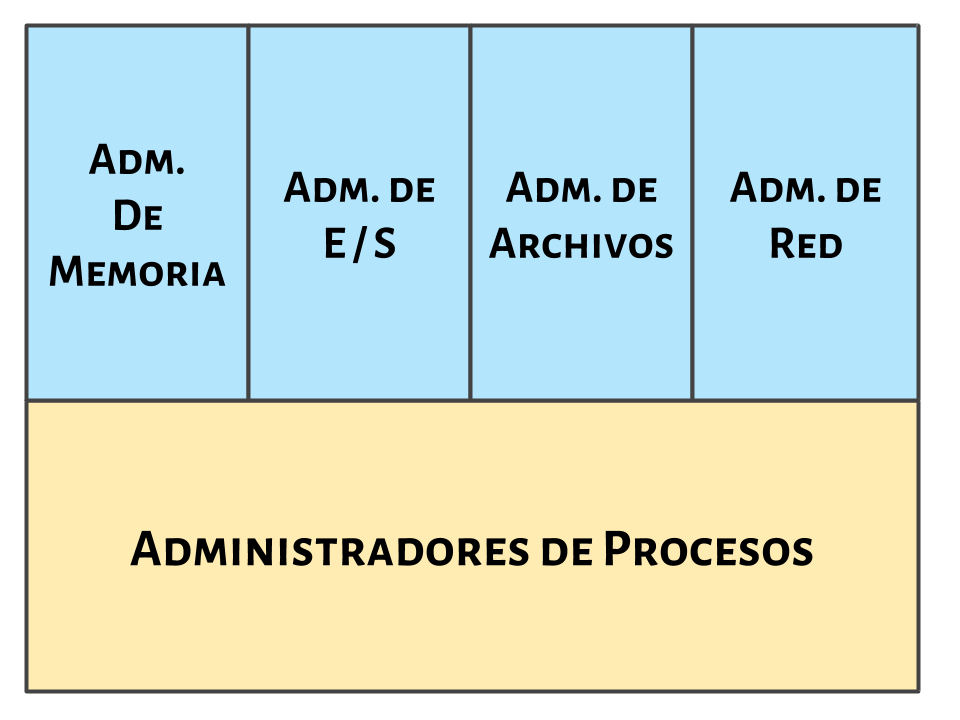
\includegraphics[width=0.35\textwidth]{PartesDelKernel}
            \end{figure}





% //////////////////////////////////////////////////////////////////////////////////////////////////////////
% ///////////////////////////         PROCESOS HILOS Y VIRTUALIZACION           ////////////////////////////
% //////////////////////////////////////////////////////////////////////////////////////////////////////////
\part{Procesos y Virtualización de CPU}
\clearpage


    % ===============================================================================
    % ====================              PROCESOS        =============================
    % ===============================================================================
    \chapter{Procesos}

        % ==============================================
        % ===========      INTRODUCCIÒN      ===========
        % ==============================================
        \clearpage
        \section{Introducción}

            % ==============================================
            % ===========       PROCESOS        ============
            % ==============================================
            \clearpage
            \subsection{Conozcamos a los Procesos}

                El Administrador de los Procesos se encarga de la gestión de cualquier trabajo
                a ejecutar en el sistema.

                La clave durante este capitulo será la virtualización, la virtualización es
                la tecnica que haremos para hacerle creer a cada \Quote{programa} que se este
                ejecutando que es el único en ejecucción y tiene siempre acceso a la CPU.


                Haremos esto porqe basicamente tenemos una pequeña cantidad de procesadores y 
                muchisimos programas intentando ejecutarse al mismo tiempo.

                Ahí esta la clave del problema... ¿Cómo podemos crear la ilusión de tener
                muchísimas CPU's?

                Vamos a introducir una de las abstracciones más fundamentales que nos da el 
                sistema operativo: Los Procesos.

                El Sistema Operativo logra crear esta ilusión de una gran cantidad de procesadores
                gracias a la virtualización de la CPU, es decir, gracias a estar corriendo un proceso
                y luego parandolo para correr el siguiente, esta tecnica es conocida como \textbf{
                tiempo compartido}.

                Pata implementar la virtualización y para implementarla bien veremos sobre algunas
                de los mecanismos a bajo nivel como \textbf{el cambio de contexto} o técnicas de 
                alto nivel como \textbf{las políticas de planificación}.

            % ==============================================
            % ===========       PROCESOS        ============
            % ==============================================
            \clearpage
            \subsection{Definición de un Proceso}

                Aquí entre amigos podemos definir a un proceso como un programa en ejecución,
                así de simple.

                Podemos diferenciar un programa en ejecución de otro por el PC, es decir, 
                por cuales instrucciones se estan ejecutando, por el valor actual de los registros,
                la pila de punteros o cosas así, así que si vamos a asbtraer / generalizar un proceso
                tendremos que tener una forma de almacenar dicha información que identifica a nuestros
                programas.

                Formalmente podemos decir que:
                \Quote{Un proceso es un programa en ejecución, es la entidad mínima de software
                ejecutándose en el sistema operativo contenido en una estructura de información}

                De esta definición podemos obtener dos características muy importantes:
                \begin{itemize}
                    
                    \item \textbf{Es una Entidad de Software}

                        Esto implica que tendrá asociado un ciclo de vida. Este ciclo representará
                        las diverdad etapas por las cuales puede transitar un proceso.

                        Un proceso en el sistema operativo se implementará a través de una
                        estructura de información, la cual contendrá toda la información necesaria
                        para caracterizar a dicho proceso.

                        Esta estructura de información es implementada mediante una
                        estructura de datos en el lenguaje de alto nivel que estemos utilizando.

                        A esta estructura se le conoce como \textbf{Bloque de Control del Proceso}
                        (PCB). 

                        Este PCB es el elemento con el que el Administrador de Procesos
                        interacturá durante el ciclo de vida del proceso presente en el sistema 
                        operativo.

                    \item \textbf{Representa una Estructura de Información}

                        Un proceso se implementa a traves de una estructura de información, la cual contendra
                        toda la información necesaria para caracterizar completamente cual proceso representado

                        Esta estructura de informacion es implementada mediante una estructura de datos en un
                        lenguaje de programacion, y se le conoce como bloque de control de proceso (PCB).
                        Este bloque es un elemento principal ya que el administrador de procesos va a estar
                        en contacto con el durante el ciclo de vida del procesos.
                    
                \end{itemize}



        % ==============================================
        % =====  BLOQUE DE CONTROL DE PROCESOS   =======
        % ==============================================
        \clearpage
        \section{Bloque de Control de Proceso (PCB)}

            La imprementación de un proceso en un sistema operativo se lleva a cabo mediante
            una estructura de datos, esta es conocida como un PCB.
            Este mantiene toda la información importante de un proceso, esta nos permite 
            caraterizar un proceso en el sistema operativo.

            Cada sistema implementa estas estructuras de manera diferente, pero en general
            todas contienen un:

            \begin{itemize}
                \item
                    \textbf{Apuntador:}

                    Mantiene un referencia del PCB en la cola de planificación

                \item
                    \textbf{Identificador:}

                    Es un simple entero positivo que se encarga identificar al proceso

                \item
                    \textbf{Contador de Programa:}

                    Mantiene el valor del registro del procesador PC ó IP, es decir, la dirección
                    de la siguiente instrucción a ejecuctar por el proceso

                \item
                    \textbf{Registros:}

                    Estos datos antienen los valores de los registros del procesador que actualmente
                    tiene el proceso en ejecuciòn.
                \item
                    \textbf{Estado del Proceso:}

                    Este dato mantiene el estado del ciclo de vida actual, en el que se encuentra
                    la ejecuciòn de un proceso.

                \item
                    \textbf{Información de Planificación:}

                        Estos datos mantienen información relacionada a la forma en que un proceso será
                        planificado, entre esta informaciòn se encuentra la siguiente: 

                            \begin{itemize}
                                \item Algoritmo de planificacion utilizado 
                                \item Prioridad del proceso (en caso de ser utilizada)
                            \end{itemize}

                \clearpage

                \item
                    \textbf{Información de Memoria:}

                        Estos datos mantienen información relacionada con la administración de memoria
                        usada para la ejecuciòn del progceso, esta información incluye lo siguiente:

                        \begin{itemize}
                            \item Páginas o segmentos usasdos por el proceso
                            \item Tabla de pàginas o segmentos utilizados por el proceso 
                        \end{itemize}
                
                \item
                    \textbf{Información de Contable:}
                    
                        Estos datos mantienen información relacionada con diferentes tiempos consmidos por
                        el proceso, entre estos tiempos se encuentran las siguientes: 
                        \begin{itemize}
                            \item Tiempo de accesso a memoria 
                            \item Tiempo de acceso a dispositivos de entrada y salida.
                            \item Tiempo de uso de la CPU
                        \end{itemize}

                \end{itemize}

                El administrador de procesos basa su operación fundamentalmente en la manipulación de los PCB
                de los procesos actualmente en ejecución en el sistema operativo, siendo su unidad básica funcional.
        


        % ==============================================
        % ===========      PROCESOS         ============
        % ==============================================
        \clearpage
        \section{La API de los Procesos}

            % ==============================================
            % ===========         VISTA GENERAL     ========
            % ==============================================
            \subsection{Vista General}

                Veremos pronto una visión particular de cada llamada el sistema, pero 
                antes te mostraré que es lo que debería venir incluido en cada interfaz
                con el sistema operativo para manejar procesos.

                \begin{itemize}
                    \item
                        \textbf{Crear Procesos:}
                        Cualquier sistemas operativo debe tener una 
                        forma de crear un proceso, esto sería la llamada usada
                        cuando ejecutas un comando o cuando das doble click en el icono
                        de una app.

                        Generalmente un sistema operativo te dará varias maneras en 
                        las cuales puedes crear un nuevo proceso, pero en todas lo
                        que ocurre tras banbalinas es basicamente lo mismo:

                        El proceso es código-instrucciones que se cargan a memoria,
                        se le va a reservar algo de memoria conocida como el stack 
                        (esa memoria que se usa para las variables locales, los 
                        parametros de una función ó los valores de retorno), seguramente
                        también se encargará de llenar los tan famosos $argc, argv$,
                        también reservará espacio para el heap, este es usado
                        para alocar memoria dinamicamente, como al llamar al $malloc()$,
                        también se encargará seguramente de abrir 3 archivos, uno para
                        errores y una entrada y salida estandar. Finalmente ahora si
                        coloca el apuntador a la instrucción actual al inicio de $main()$
                        por lo que el proceso-programa ahora tiene el control de la CPU.

                    \item
                        \textbf{Destruir Procesos:}
                        Cualquier sistemas operativo debe tener una 
                        forma de matar un proceso, esto sería la llamada usada
                        cuando nuestro pequeño procesos hace algo que no debe como
                        tomar memoria que no es suya o cuando un proceso bonito finalizo
                        sin mas problemas.

                    \item
                        \textbf{Esperar Procesos:}
                        Muchas veces será útil tener una forma de tomar un proceso
                        en ejecución y pasarlo a un estado de \Quote{idle} en el
                        que podemos poner en ejecución otro proceso.

                    \item
                        \textbf{Información del Procesos:}
                        Muchas veces será útil tener una forma de saber la información
                        personal de cada proceso, cuanto tiempo ha usado al CPU, cual
                        es el ID de su proceso padre o en que estado esta actualmente.
                 \end{itemize} 


            % ==============================================
            % ===========         VISTA GENERAL     ========
            % ==============================================
            \clearpage
            \subsection{Crear Procesos con $fork()$}

                Es bastante obvio que $fork()$ nos permitirá crear procesos,
                pero creeme si te digo que es la llamada a sistema más rara que has visto
                nunca.

                Antes que nada, es importante recordar que para el sistema operativo
                todo proceso tiene un ID, ó PID, este se obtiene muy fácil con $getpid()$

                Lo que hará esta llamada al sistema es crear un nuevo proceso, completamente
                nuevo, pero a imagen y semejanza del proceso actual, un proceso hijo
                si lo quieres ver así. Todo será igual, excepto algo:

                \begin{itemize}
                    \item El proceso padre obtendrá el PID del proceso hijo como valor
                        de retorno del $fork()$
                    \item El proceso hijo obtendrá un 0 como valor de retorno del
                    $fork()$, además de ser la línea de código siguiente desde la cual
                    va a empezar a correr.
                \end{itemize}

                Y si somos extrictos, si algo fallará entonces $fork()$ nos regresa
                un lindo valor negativo.

                Ahora otra cosa que ver es que ahora, nuestro resultado no será deterministico
                porque no sabemos que se ejecutará primero, si el proceso padre o el hijo, 
                ni cuanto tiempo parasá entre la ejecución de uno y de otro.

                % ========================================
                % ===========        CODE         ========
                % ========================================
                \subsubsection{Ejemplo}
                    \begin{lstlisting}[language=C, gobble=24]
                        /*=======================================================================
                        =================       FORK SYSTEM CALL    =============================
                        =========================================================================
                            USE: $ C99 Fork.c && reset && ./a.out
                        */

                        #include <stdio.h>                                                  //We will need this
                        #include <stdlib.h>                                                 //We will need this        
                        #include <unistd.h>                                                 //We will need this        
                        #include "SuperSimpleErrorHandling.c"                               //My simple code :p


                        // ==========================================
                        // ======      MAIN FUNCTION       ==========
                        // ==========================================
                        int main(int argc, char *argv[]) {                                  //This is fucking main
                            printf("Hello World \t\t(PID %i)\n", getpid());                 //Show me your ID
                            
                            int ChildID = fork();                                           //Now create a new process
                            if (ChildID < 0) return ShowError("Error at Fork", 1);          //Go an show it

                            if (ChildID == 0)                                               //YOU ARE THE CHILD?
                                printf("I am Child \t\t(PID %i)\n", getpid());              //Show me your ID then kid
                            else                                                            //YOU ARE THE PARENT
                                printf("I'm Parent of %d \t(PID %i)\n", ChildID, getpid()); //Show me your ID then old man

                            return 0;
                        }
                    \end{lstlisting}


            % ==============================================
            % ===========         VISTA GENERAL     ========
            % ==============================================
            \clearpage
            \subsection{Esperar a Procesos Hijos con $wait()$ y $waitpid()$}

                Ya que hemos creado varios procesos nos vemos en un problema algo grave:
                Ya que el orden en el que se ejecutan dichos procesos no depende de 
                nosotros sino de los algoritmos de planeación sobre la CPU no podemos
                asegurar en ningun momento si el código que estamos escribiendo sobre
                un proceso se estará ejecutando antes o después de que terminan sus 
                procesos hijos.

                Si quisieramos asegurarnos de esto entonces tenemos dos llamadas al
                sistema muy muy interesantes:

                \begin{itemize}
                    \item $wait()$: Espera a todos los procesos hijos
                    \item $waitpid(ChildXPID)$: Espera a proceso con
                        el PID que le pasemos
                \end{itemize}


            % ==============================================
            % ===========         VISTA GENERAL     ========
            % ==============================================
            \clearpage
            \subsection{Crear Procesos son $exec()$}

                Ya vimos $fork()$ que era la manera más rara de crear procesos
                pues nos permitia crear varias \Quote{copias} del mismo programa
                en diferentes procesos.

                Pero no siempre queremos eso, a veces querremos crear un proceso
                con un programa completamente diferente. 

                % ========================================
                % ===========        VERSIONES    ========
                % ========================================
                \subsection{¿Porque hay tantas Llamadas al sistema del estilo $exec*()$}

                    Ok, ok, antes de avanzar mas adelante tengo que contarte algo que
                    a mi me tiene muy sorprendido es la gran cantidad de llamadas
                    al sistema que hay con este estilo, son 5:
                    $execl()$, $execle()$, $execlp()$, $execv()$, $execvp()$.

                    Ahora empecemos, con porque tienen esos nombres tan raros:

                    \begin{itemize}
                        \item \textbf{L vs V}:
                            Define la cantidad de parametros que quieres pasarle al
                            nuevo proceso.

                            \begin{itemize}
                                \item \textbf{L} si es que solo te interesa pasar uno
                                como en $execl(), execle(), execlp()$

                                \item \textbf{V} si es que solo te interesa pasar es
                                un arreglo de char* como en $execv(), execvp()$
                            \end{itemize}

                            El formato por array es muy util cuando el número
                            de parametros que vas a enviar al proceso es variable.


                        \item \textbf{E}:
                            Las versiones con una e al final le permiten, además,
                            pasar un array de char* que son un conjunto de cadenas añadidas al entorno de procesos generado antes de que se inicie el programa ejecutado.

                            En realidad es otra forma de pasar parámetros.

                        \item \textbf{P}:
                            Las versiones que NO la llevan requieren un path absoluto
                            o relativo hacia donde esta el ejecutable si es que no
                            esta en el directorio de trabajo.

                    \end{itemize}

                % ==============================================
                % ===========    SUSTITUCON DE CODIGO   ========
                % ==============================================
                \subsection{Sustitución de Código}

                    Decimos que $exec()$ crea procesos mediante la sustitución de código, es decir:
                    \begin{itemize}
                        \item El nuevo proceso sustituye y destruye al proceso padre
                        \item La memoria utilizada por el proceso creador es reutilizada por el nuevo
                        proceso
                    \end{itemize}

                % ========================================
                % ===========        CODE         ========
                % ========================================
                \clearpage
                \subsubsection{Ejemplo}
                    \begin{lstlisting}[language=C, gobble=24]
                        /*=======================================================================
                        =================       EXEC SYSTEM CALL    =============================
                        =========================================================================
                            USE: $ C99 Exec.c && reset && ./a.out
                        */

                        #include <stdio.h>                                                  //We will need this
                        #include <stdlib.h>                                                 //We will need this        
                        #include <sys/wait.h>                                               //We will need this  
                        #include <unistd.h>                                                 //We will need this        
                        #include <string.h>                                                 //We will need this        
                        #include "SuperSimpleErrorHandling.c"                               //My simple code :p

                        int main(int argc, char *argv[]) {                                  //Fucking main
                            printf("Hello World \t\t\t(PID %i)\n", getpid());               //Show me your ID

                            int ChildID = fork();                                           //Now create a new process
                            if (ChildID < 0) ShowErrorAndGo("Error at Fork", 1);            //Go an show it

                            if (ChildID == 0) {                                             // === YOU ARE THE CHILD =====
                                printf("I am Child \t\t\t(PID %i)\n", getpid());            //Show me your ID then kid

                                char *Arguments[3];                                         //Create an array of strings :D
                                Arguments[0] = strdup("wc");                                //New program: "wc" (word count)
                                Arguments[1] = strdup("Exec.c");                            //Argument to wc: file to count
                                Arguments[2] = NULL;                                        //End of array
                                execvp(Arguments[0], Arguments);                            //Run wc & 'exit' process
                                
                                printf("This shouldn't print out ever :o");                 //All this code stop existing
                            }
                            else {                                                          // ==== YOU ARE THE PARENT ====
                                int WCID = wait(NULL);                                      //This return the pid of the child
                                printf("I'm Parent of %i aka wc-%i", ChildID, WCID);        //Show me your ID then old man
                                printf("\t(PID %i)\n", getpid());                           //Show me your ID then old man
                            }
                            return 0;
                        }

                    \end{lstlisting}



        % ==============================================
        % =====        ARBOL DE PROCESOS         =======
        % ==============================================
        \clearpage
        \section{Árbol de Procesos}

            Internamente, un administrador de procesos utiliza una estructura no lineal para organizar todos
            los procesos actualmente en ejecución, esta estructura no lineal es conocidada como árbol de procesos.

            Un árbol de procesos esta formado por un nodo raíz conocido como proceso principal, cada sistema
            operativo nombra a este proceso principal de forma particular, sin embargo, la funciòn de este proceso
            es la misma, funciona como la base para la creación de cualquier proceso en el sistema operativo.

            El arbol de procesos clasifica los procesos en dos tipos:

            \begin{itemize}
                \item
                    \textbf{Proceso de Sistema}

                    Los procesos de sistema son aquellos que conforman al sistema operativo, se caracterizan
                    por ejecutarse en un modo nodo del procesador conocido como modo kernel.
                    En el modo kernel de un procesador se tiene permitido el acceso sin algùn tipo de reztrición
                    a cualquier recurso del procesador y del equipo de còmputo.


                \item
                    \textbf{Proceso de Usuario}

                    Los procesos de usuario son todos aquellos procesos ejecutados por los usuarios del sistema
                    operativo, se caracterizan por ejecutarse en un modo del procesador conocido como modo usuario.

                    En el modo usuario de un procesador se restringe el acceso a recursos cróticos tanto del
                    procesador como del equipo de cómputo.

            \end{itemize}

            En el Árbol de Procesos se le asigna un identificador para referenciar a los procesos, este
            identificador es un valor entero positivo único, que se asigna una vez que se crea el proceso.
            Cualquier referencia se lleva acabo a través de este indentificador.

            Dentro de este Árbol se establece una relación Hijo-Padre entre los procesos, esta relación 
            permite heredar características de un proceso padre a sus hijos, además nos permite mantener
            una organización centralizada.

            Esto nos dice que no existen procesos aislados, todo proceso tiene que estar contenido en el
            Árbol de Procesos.



    % ===============================================================================
    % ====================      PLANIFICACION DE PROCESOS        ====================
    % ===============================================================================
    \chapter{Planificación de Procesos}


        % ==============================================
        % ===========    PROCESOS EN C      ============
        % ==============================================
        \clearpage
        \section{Planificación de Procesos}



            % ==============================================
            % ===========    SUSTITUCON DE CODIGO   ========
            % ==============================================
            \subsection{Tipos de Planificación}

                Consiste en la seleccion de uno o mas procesos presentes en el sistema operativo para asignarles
                un recurso requerido. Existen 3 tipos:

                \begin{itemize}
                    \item
                        \textbf{Planificación a Largo Plazo:}

                        Selecciona procesos del disco duro para colocarlos en la memoria física:
                        \begin{itemize}
                            \item Tiene el tiempo de ejecucion mas lento
                            \item Presente principalmente en los sistemas operativos por lotes
                        \end{itemize}

                    \item
                        \textbf{Planificación a Mediano Plazo:}

                        Selecciona procesos del la memoria virtual para colocarlos en la memoria física:
                        \begin{itemize}
                            \item Mas rápido que la planeación a largo plazo
                            \item Presente en sistemas operativos con multiprogramacion y tiempo compartido
                            \item Estos dos tipos de planificacion definen el grado de multiprogramacion que tiene
                                un sistema operativo, es decir el grado de multiprogramacion es el número máximo
                                de procesos que pueden colocarse en la memoria física simúltaneamente
                        \end{itemize}

                    \item
                        \textbf{Planificación a Corto Plazo:}

                        Selecciona procesos para colocarlo directamente el la CPU:
                        \begin{itemize}
                            \item Mas rápido que todas
                            \item Presente en sistemas operativos gracias al despachador
                        \end{itemize}

                \end{itemize}


            % ==============================================
            % ===========       DESPACHADOR         ========
            % ==============================================
            \clearpage
            \subsection{Despachador}

                Elemento del administrador de procesos que lleva a cabo el cambio de contexto de la CPU, 
                son de tamañno reducido de hasta 256Kb con tiempos de ejecución contado normalmente en
                nanosegundo.

                Decimos que estamos cambiando de contexto cuando se desaloja el proceso que está en el CPU,
                previo respaldo del estado actual de ejecución del proceso, y colocar otro proceso en la CPU
                para iniciar o continuar su ejecución.

                \subsubsection{Características}

                \begin{itemize}
                    \item Cambia la CPU de modo usuario a modo kernel
                    \item Respalda el contexto del proceso actual en su PCB respectivo
                    \item Desaloja el proceso actual
                    \item Inicia el contexto del proceso a iniciar por medio de su PCB
                    \item Inicia el PC o IP con las siguientes instrucciones a ejecutar
                    \item Cambia la CPU de modo kernel a modo usuario
                \end{itemize}


            % ==============================================
            % ======   ALGORITMO DE PLANIFICACION     ======
            % ==============================================
            \clearpage
            \subsection{Algoritmo de Planificación}


                Los algoritmos permiten la selección de un proceso bajo algun criterio de planificación
                respectivo a la cola, para asi asignarle algun recurso requerido.

                Todos estos algoritmos se aplican a la cola de planificacion, que es donde se agrupa
                todos los procesos que solicitan el uso de algún recurso.

                \subsubsection{Tipos}

                \begin{itemize}
                    \item Primero en Llegar Primero en Servirse (FCFS)
                    \item Primero el Trabajo mas corto (SJF)
                    \item Algoritmo por Prioridad
                    \item Algoritmo por Torno Circular (Round Robin)
                \end{itemize}


            % ==============================================
            % ===========    SUSTITUCON DE CODIGO   ========
            % ==============================================
            \subsection{Colas de Múltiplos Niveles}

                Es como se implementan las colas de planificacion en los sistemas operativos, pues estas estan
                asociada a una subcola, existen dos tipos:

                \begin{itemize}
                    \item
                        \textbf{Cola de Múltiples Niveles Simple:}

                        Cada que un proceso se asigna a una subcola bajo ninguna circustancia puede ser cambiada
                        a otra subcola.

                    \item
                        \textbf{Cola de Múltiples Niveles Retroalimentada:}

                        Cualquier proceso se asigna a una subcola puede ser cambiada
                        a otra subcola.

                \end{itemize}


                Recuerda que cada subcola puede tener un algoritmo propio, además de tener un algoritmo
                global que nos permita administrar a cola global.


            % ==============================================
            % =====    COMUNICACION ENTRE PROCESOS  ========
            % ==============================================
            \subsection{Comunicación entre Procesos}

                Los procesos desde el punto de vista de la comunicación pueden clasificarse en dos tipos:

                \begin{itemize}
                    \item \textbf{Procesos Independientes:}
                        Estos son aquellos que no requieren comunicación con otros procesos para completar
                        su ejecución.

                    \item \textbf{Procesos Cooperativos:}
                        Estos necesitan la comunicación para poder completar su ejecución

                        Estos requieren la ayuda del sistema operativo para poder llevar a cabo la comunicación,
                        esto se hace mediante los procesos conocidos como IPC (Comunicación Inter Procesos).
                \end{itemize}

            % ==============================================
            % ===========         IPC       ================
            % ==============================================
            \clearpage
            \subsection{IPC}

                \begin{itemize}
                    \item \textbf{Tuberías}: Son archivos creados y controlados internamente por el 
                        sistema operativo, sirven como buffers en los cuales se almacenan los datos
                        a comunicar. implementan primitivas para la lectura y escritura de datos.

                        A final de cuentas es un archivo que crea el sistema operativo, por lo tanto
                        podemos usar las llamadas al sistema que usamos para archivos.

                        Los mensajes a comunicar se manejan como mensajes sin formato. Unicamente soportan
                        comunicación unidireccional con una conectividad uno a uno.

                    \item \textbf{Memoria Compartida}:
                        Es una región de memoria creada y controlada por el sistema operativo asociada a un
                        proceso, la región de memoria creada se anexa al espacio de direcciones del proceso
                        que utilizará la memoria compartida.

                        Se accede a ella mediante un apuntador a esa región. La memoria compartida puede ser
                        accedida por todos los procesos que lo necesiten.

                        Por su naturaleza necesitamos tener una forma de sincronizar toda la información.

                    \item \textbf{Sockets}:
                        Son parecidos a la tuberías, sin embargo su implementación se apoya en el administrador
                        de red.

                        Todos los mensajes tiene un formato estandarizado, ya que se apoyan con el administrador
                        de red, podemos comunicar procesos de manera local y de manera remota.

                        El administrador de red es el que se encarga de seleccionar el protocolo que se hará entre
                        los mensajes.

                        Recuerda que el socket es bidireccional.

                        Debido justo a que tienen un protocolo son más lentos que las tuberías.
                \end{itemize}




% //////////////////////////////////////////////////////////////////////////////////////////////////////////
% ///////////////////////////         PROCESOS HILOS Y VIRTUALIZACION           ////////////////////////////
% //////////////////////////////////////////////////////////////////////////////////////////////////////////
\part{Hilos y Virtualización de Memoria}
\clearpage


    % ===============================================================================
    % ====================              HILOS           =============================
    % ===============================================================================
    \chapter{Abstracción de Memoria}

        % ==============================================
        % ===========      INTRODUCCIÒN      ===========
        % ==============================================
        \clearpage
        \section{Espacio de Direcciones}

            Antes que nada, recuerda, al Sistema Operativo le importa virtualizar cualquier recurso del pc,
            eso no solo quiere decir que van a virtualizar la CPU, sino también la memoria, así que grabate eso
            muy bien, pero muy bien, TODA DIRECCIÓN DE MEMORIA DENTRO DE UN PROGRAMA ES UNA DIRECCIÓN VIRTUAL.

            Podemos dividir la abstracción que nos da el Sistema Operativo en 3 partes:

            \begin{itemize}
                \item \textbf{Zona del Codigo}: Es literal la sección en la que esta el codigo, es aquí por
                ejemplo a donde van los punteros a funciones.

                \item \textbf{Stack}: Conocido también como pila, es la parte que se encarga de que mantener
                la información de las cadenas de llamadas a funciones, es la que se usa cuando se crean variables
                locales.

                Es conocida a veces como la memoria automatica, porque cuando por ejemplo tu declaras
                una variale en una función el compilador se encarga de reservar espacio para ella y de
                liberarla cuando se sale de la función.

                \item \textbf{Heap}: Es la que se encarga de las variables que se crean dinamicamente.
                Por ejemplo de es la memoria que se reserva cuando se llama a $malloc()$

            \end{itemize}


            % ========================================
            % ===========        CODE         ========
            % ========================================
            \subsubsection{Ve donde esta tu Memoria Virtual}
                \begin{lstlisting}[language=C, gobble=20]
                    /*=======================================================================
                    =================       WHERE IS MEMORY     =============================
                    =========================================================================
                        USE: $ C99 CodeStackAndHeap.c && reset && ./a.out                  */
                    #include <stdio.h>                                              //We will need this
                    #include <stdlib.h>                                             //We will need this        

                    int main(int argc, char *argv[]) {                              //Fucking main
                        int LocalVariable;                                          //A var in stack
                        printf("Location of Code:  %p\n", (void *) main);           //Show direction for code
                        printf("Location of Heap:  %p\n", (void *) malloc(1));      //Show direction for heap
                        printf("Location of Stack: %p\n", (void *) &LocalVariable); //Show direction for stack
                        
                        return 0;                                                   //Go little program
                    }
                \end{lstlisting}


                    

    % ===============================================================================
    % ====================              HILOS           =============================
    % ===============================================================================
    \chapter{Hilos aka Procesos Ligeros}

        % ==============================================
        % ===========      INTRODUCCIÒN      ===========
        % ==============================================
        \clearpage
        \section{Introducción}

            Son procesos ligeros, es una alternativa a las aplicaciones concurrentes.

            Un hilo es un componente de un proceso tradicional que se ejecuta en concurrencia con
            sus proceso creador.

            Para el sistema operativo es más facil crear hilos que crear un proceso tradicional, por eso se
            le llaman procesos ligeros.

            \begin{itemize}
                \item Comparten valores de los recursos asignados a su proceso creador,
                    siendo la memoria (heap) el principal recurso compartido. Nota, dije que comparten
                    el heap, osea es donde se encuentras las variables que se crean mediante malloc o
                    dinamicamente.

                \item Manejan de manera independiente tanto la pila como el stack
                
                \item Dependen de la ejecución de su proceso padre, el cual es un proceso tradicional

            \end{itemize}

        % ==============================================
        % ===========      HILOS            ============
        % ==============================================
        \clearpage
        \section{La API de los Hilos}

            % ==============================================
            % ===========      CREACION DE HILOS     =======
            % ==============================================
            \subsection{Estructura de Hilos General}

                Para poder interactuar con el hilo usaremos una estructura $pthread_t$


            % ==============================================
            % ======      CREAR HILOS      =======
            % ==============================================
            \subsection{Creación de Hilos}

                % ========================================
                % ===========        CODE         ========
                % ========================================
                \subsubsection{Ejemplo de la Declaración}
                    \begin{lstlisting}[language=C, gobble=24]
                        #include <pthread.h>
                        int
                        pthread_create( pthread_t *       ThreadID,
                                        const pthread_attr_t *  Attributes,
                                        void *            (*Function)(void*),
                                        void *            Argument)
                    \end{lstlisting}

                    Veamos cada uno de los parametros:
                    \begin{itemize}
                        \item $ThreadID$ es un puntero a la estructura del archivo
                        \item $Attributes$ son los atributos que tendrá el hilo, pero de forma
                            general un $NULL$ será mas que suficiente por default
                        \item $Function$ es la función que ejecutará el hilo, que recibe 
                            un puntero generico como parametro y regresará un puntero generico como
                            resultado.
                        \item $Argument$ es exactamente el que le vas a pasar como argumento
                    \end{itemize}


            % ==============================================
            % ======        COMPLETAR HILOS          =======
            % ==============================================
            \subsection{Esperar Hilos}

                Si te gustaría esperar que acabe un hilo antes de continuar la ejecucción del
                codigo basta con hacer algo como:

                % ========================================
                % ===========        CODE         ========
                % ========================================
                \subsubsection{Ejemplo de la Declaración}
                    \begin{lstlisting}[language=C, gobble=24]
                        #include <pthread.h>
                        int
                        pthread_join(   pthread_t *       ThreadID,
                                        void **           Value)
                    \end{lstlisting}

                    Veamos cada uno de los parametros:
                    \begin{itemize}
                        \item $ThreadID$ es un puntero a la estructura del archivo
                        \item $Value$ es un puntero al valor de retorno que tu esperas
                        osea un puntero a un puntero generico
                    \end{itemize}





\end{document}










